\let\negmedspace\undefined
\let\negthickspace\undefined
\documentclass[journal]{IEEEtran}
\usepackage[a5paper, margin=10mm, onecolumn]{geometry}
%\usepackage{lmodern} % Ensure lmodern is loaded for pdflatex
\usepackage{tfrupee} % Include tfrupee package

\setlength{\headheight}{1cm} % Set the height of the header box
\setlength{\headsep}{0mm}     % Set the distance between the header box and the top of the text

\usepackage{gvv-book}
\usepackage{gvv}
\usepackage{cite}
\usepackage{amsmath,amssymb,amsfonts,amsthm}
\usepackage{algorithmic}
\usepackage{graphicx}
\usepackage{textcomp}
\usepackage{xcolor}
\usepackage{txfonts}
\usepackage{listings}
\usepackage{enumitem}
\usepackage{mathtools}
\usepackage{gensymb}
\usepackage{comment}
\usepackage[breaklinks=true]{hyperref}
\usepackage{tkz-euclide} 
\usepackage{listings}
% \usepackage{gvv}                                        
\def\inputGnumericTable{}                                 
\usepackage[latin1]{inputenc}                                
\usepackage{color}                                            
\usepackage{array}                                            
\usepackage{longtable}                                       
\usepackage{calc}                                             
\usepackage{multirow}                                         
\usepackage{hhline}                                           
\usepackage{ifthen}                                           
\usepackage{lscape}
\usepackage{circuitikz}


\begin{document}

\bibliographystyle{IEEEtran}
\vspace{3cm}

\title{2.10.12}
\author{AI25BTECH11023-Pratik R}
 \maketitle
% \newpage
% \bigskip
{\let\newpage\relax\maketitle}

\renewcommand{\thefigure}{\theenumi}
\renewcommand{\thetable}{\theenumi}
\setlength{\intextsep}{10pt} % Space between text and floats


\numberwithin{equation}{enumi}
\numberwithin{figure}{enumi}
\renewcommand{\thetable}{\theenumi}

\textbf{Question}:\\
A unit vector perpendicular to the plane determined by the points
$P\brak{1,-1,2}$,$Q\brak{2,0,-1}$ and $R\brak{0,2,1}$ is \\ 
\textbf{solution}: \\
According to the question, \\
Given the position vectors,
\begin{align}
    \vec{P}=\myvec{1\\-1\\2};
    \vec{Q}=\myvec{2\\0\\-1};
    \vec{R}=\myvec{0\\2\\1}
\end{align}


Let the perpendicular vector be $\vec{n}^T=\myvec{n_1&&n_2&&n_3}$
\begin{align}
    \because \vec{n}^\top \vec{P}=1\\
    \vec{n}^\top \vec{Q}=1 \\
    \vec{n}^\top \vec{R}=1
\end{align}
\begin{align}
    \therefore \myvec{\vec{P}^\top \\\vec{Q}^\top \\\vec{R}^\top}\vec{n}= \myvec{1 \\ 1}
\end{align}
\begin{align}
    \therefore \myvec{\vec{P} & \vec{Q} & \vec{R}}^\top \vec{n}= \myvec{1 \\ 1}
\end{align}
\begin{align}
    \myvec{1&&-1&&2\\2&&0&&-1 \\ 0&&2&&1} \vec{n}= \myvec{1 \\ 1 \\ 1}
\end{align}
The augmented matrix for the above system of Equations is given by
\begin{align}
    \myvec{1&-1&2&&1\\2&0&-1&&1\\0&2&1&&1} 
\end{align}

Solving equation 0.8 we get
\begin{align}
    \vec{n}=\myvec{\frac{2}{3}\\\frac{1}{3}\\\frac{1}{3}}
\end{align}


The unit vector perpendicular to the plane is given by \vec{x}\\
\begin{align}
     \vec{x}= \frac{\vec{n}}{||n||} =   \frac{1}{\sqrt{6}}\myvec{2\\1\\1}
\end{align}
\\

\begin{figure}[H]
    \centering
    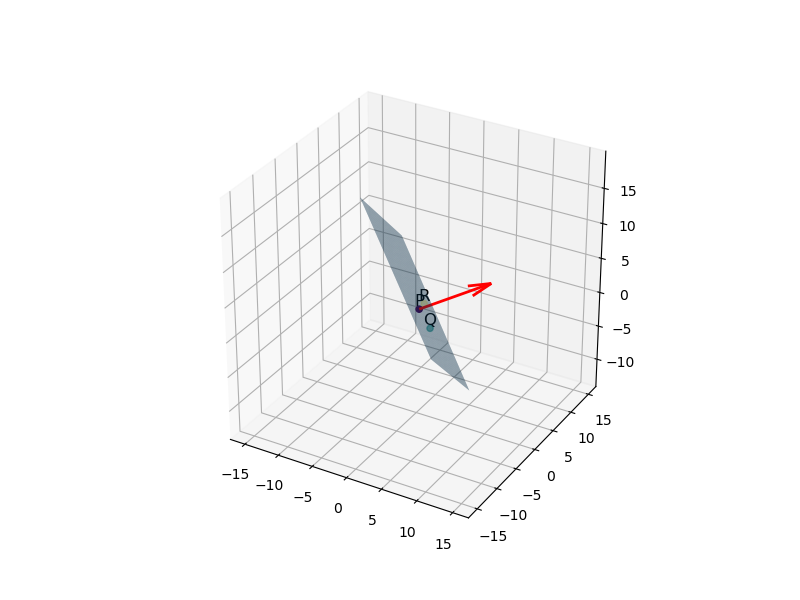
\includegraphics[width=0.8\columnwidth]{figs/fig.png}
    \label{fig-1}
\end{figure}

 


\end{document}